\section{Appendix to Section 4 --  Fundamental Concepts }
\label{app:aux}

Lemma \ref{lemma:orig:to:bounded:front} says, essentially,  that \scoped executions describe the same set of executions as those  starting at an initial state\footnote{An \emph{Initial} state's heap contains a single object of class \prg{Object}, and
its  stack   consists of a single frame, whose local variable map is a mapping from \prg{this} to the single object, and whose continuation is  any statement.
(See Def. \ref{def:initial})}.   
For instance, revisit  Fig. \ref{fig:illusrPreserve} , and assume that $\sigma_6$ is an initial state.
We have  $\leadstoOrigStar {\Mtwo} {\sigma_{10}}  {\sigma_{14}}$ and $ \notLeadstoBoundedStar {\Mtwo}  {\sigma_{10}} {\sigma_{14}}$, but also 
 $\leadstoBoundedStar  {\Mtwo}  {\sigma_{6}}   {\sigma_{14}}$. %  -- \cf Lemma  

 \begin{lemma}
\label{lemma:orig:to:bounded:front}
For all modules $\overline M$, state  $\sigma_{init}$,  $\sigma$, $\sigma'$, where
$\sigma_{init}$ is  initial:
\begin{itemize} % {enumerate} 
\item 
\label{otbOne}
$\leadstoBoundedStar  {\Mtwo}  {\sigma} {\sigma'} \ \ \Longrightarrow \  \
\leadstoOrigStar {\Mtwo} {\sigma}  {\sigma'}$
\item 
\label{otbTwo}
$\leadstoOrigStar {\Mtwo} {\sigma_{init}}  {\sigma'}  \ \  \Longrightarrow\ \
\leadstoBoundedStar  {\Mtwo}  {\sigma_{init}} {\sigma'}$.
\end{itemize}
\end{lemma}

\vspace{.05cm}

{Lemma \ref{l:var:unaffect} says that scoped execution does not affect the contents of variables in earlier frames.}
and that 
the interpretation of a variable remains unaffected by
scoped execution of statements  which do not mention that variable. More  in Appendix~\ref{app:aux}.

\begin{lemma}
\label{l:var:unaffect}
For any modules $\Mtwo$, states $\sigma$, $\sigma'$,  variable $y$, and number $k$:
\begin{itemize}
\item
\label{carInFrame}
{$\leadstoBoundedStar {\Mtwo}  {\sigma}  {\sigma'}  \ \wedge \ k<\DepthSt \sigma  \ \ \Longrightarrow \ \  \interpret {\RestrictTo \sigma k} y =  \interpret {\RestrictTo {\sigma'} k} y$
}
\item
$\leadstoBoundedStarFin {\Mtwo}  {\sigma}  {\sigma'} \ \wedge \ y\notin \vs(\sigma.\prg{cont}) \ \ \Longrightarrow \ \  \interpret \sigma y =  \interpret {\sigma'} y$
\end{itemize}
\end{lemma}

\begin{figure}[htb]
\begin{tabular}{|c|c|c|}
\hline 
\resizebox{3.5cm}{!}{
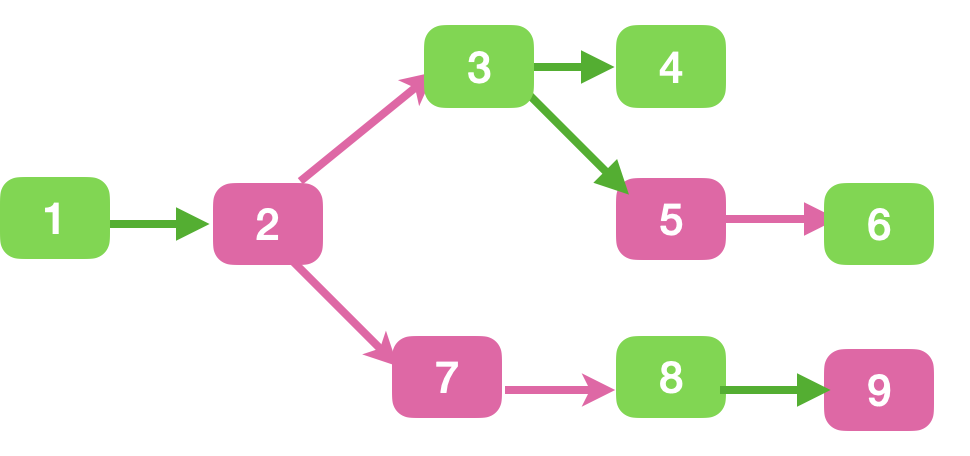
\includegraphics[width=\linewidth]{diagrams/heap.png}
} 
&
\resizebox{5cm}{!}{
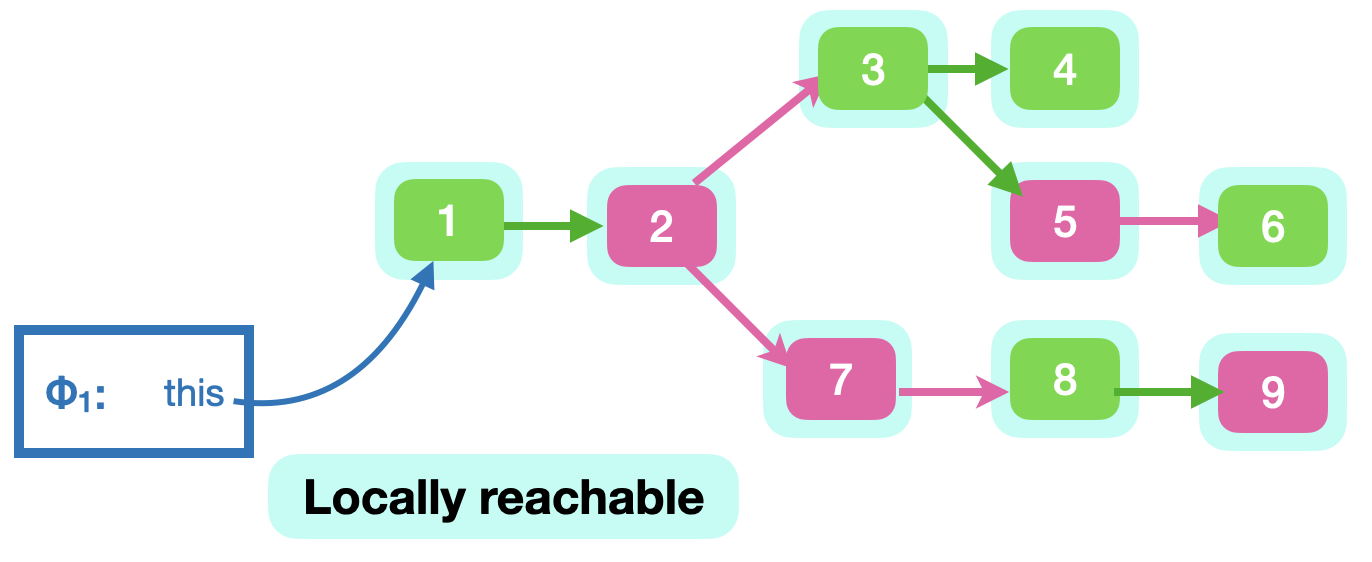
\includegraphics[width=\linewidth]{diagrams/locReachA.png}
} 
&
\resizebox{5cm}{!}{
\includegraphics[width=\linewidth]{diagrams//locReachb.png}
} 
\\
\hline
 a heap
&
Locally Reachable from $\phi_1$
&
Locally Reachable from $\phi_2$
\\
\hline \hline
\end{tabular}
   \caption{-Locally Reachable Objects} % from $\phi_1$ and $\phi_2$. } % n later chapters}
   \label{fig:LReachable}
 \end{figure}

Fig. \ref{fig:LReachable} illustrates local reachability:  In the middle pane the top frame is $\phi_1$ which maps \prg{this} to $o_1$; all objects are locally reachable. 
In the right pane the top frame is $\phi_2$, which maps \prg{this} to $o_3$, and $x$ to $o_7$; now $o_1$ and $o_2$ are no longer locally reachable.


%removed lemmas -- parts thereof are in main.
% And they are not used anyway 
%Lemma \ref{lemma:orig:to:bounded}  states that
% any execution  which is part of an execution which started at some initial state, is scoped by that state.
% 
%  \begin{lemma}
%\label{lemma:orig:to:bounded}
%For all $\overline M$, all $n,m\in \mathbb{N}$ with $m\leq n$, $\sigma_0$, ... $\sigma_n$,  $\sigma_{init}$, $\sigma$, $\sigma'$, where
%$\sigma_{init}$ is an initial state:
% \label{otbTwo}
%\[\leadstoOrigStar {\Mtwo} {\sigma_{init}}  {\sigma}\ \wedge\ \leadstoOrigStar {\Mtwo} {\sigma}  {\sigma'}\ \ \Longrightarrow\ \  \leadstoBoundedStarThree {\Mtwo} {\sigma} {\sigma_{init}} {\sigma'}\].
% \end{lemma}
% \begin{tabular}{lll}
%\begin{minipage}{.5\textwidth}
%Revisit  Fig. \ref{fig:UpSemantics} (copied here), and assume that $\sigma_6$ is an initial state where
%an initial state's heap contains a single object of class \prg{Object}, and
%its  stack   consists of a single frame, whose local variable map is a mapping from \prg{this} to the single object, and whose continuation is  any statement. 
%%(See Definition %s \ref{def:initial} and  \ref{def:arising} and the {appendices %of the full paper \cite{necessityFull}}.
%\end{minipage}
%& \ \  \   &
%\begin{minipage}{.45\textwidth}
%\begin{tabular}{|c|}
% \hline %  \\ -- this added one vertical space
%\resizebox{6cm}{!}{
%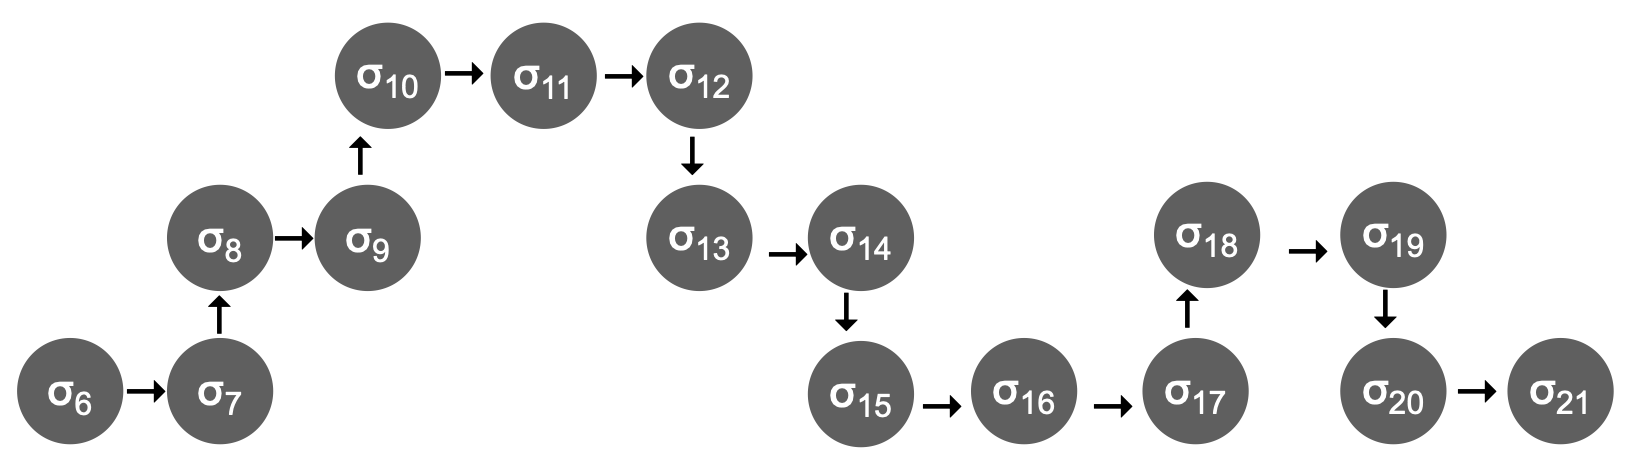
\includegraphics[width=\linewidth]{diagrams/bounded2.png}
%} 
% \\
%\hline
%
%\end{tabular}
%
%\end{minipage}
%\end{tabular}
%We have  $\leadstoOrigStar {\Mtwo} {\sigma_{10}}  {\sigma_{14}}$ and $ \notLeadstoBoundedStar {\Mtwo}  {\sigma_{10}} {\sigma_{14}}$.
%However, because $\sigma_6$ is an initial state, we have $\leadstoBoundedStarThree {\Mtwo}  {\sigma_{10}} {\sigma_{6}}  {\sigma_{14}}$ -- \cf Lemma \ref{lemma:orig:to:bounded}.
%
%%%%%%%%%%%%%%%%%%
%Lemma \ref{lemma:call:return}
%states that method calls  correspond  to pushing of frames (here $\sigma_2 \in \PushS  {\interpret {\sigma_1} {y}} {\sigma_1}$),
% that they leave the values of the caller's local variables unmodified ($\forall z. \interpret {\sigma_1} {z} = \interpret {\sigma_4} {z}$), and
%method returns  correspond  to popping  a frame  (here $\sigma_3 \in  \PushSLong  {( {\interpret {\sigma_1} {y}},{\overline \alpha})} {\sigma_4}$), where the local map of the frame being popped contains the original arguments ($\overline {{\interpret {\sigma_1} {y}}}$) as well as some additional addresses ($\overline \alpha$).
%The latter property -- that  the frame being popped from $\sigma_3$ contained the original arguments passed in to $\sigma_2$ -- holds because 
% we forbid assignments to formal parameters (but we do allow  assignments to the other local variables).
% 
% 
% \begin{lemma}
% \label{lemma:call:return}
% For any modules $\Mtwo$, states $\sigma_1$, $\sigma_2$, $\sigma_3$, and $\sigma_4$, variables $x$, $y_0... y_n$:
% 
% $  
%   \left. %\{
%   \begin{array}{l}  \ \strut \ \ \sigma_1.\prg{cont}\txteq x:= y_0.m(y_1,...y_n);\_ ,\\
%    \ \strut \ \  \leadstoOrig {\Mtwo} {\sigma_1}   {\sigma_2} , \\
%     \ \strut \ \  \leadstoBoundedStarFin  {\Mtwo}  {\sigma_2}  {\sigma_3}, \\
%  \ \strut \ \  \leadstoOrig {\Mtwo} {\sigma_3}   {\sigma_4}, 
%    \end{array} 
%\right \}
% \mbox{implies} \ \ 
%  \begin{cases}
%     \ \strut \ \  \sigma_2 \in \PushS  {\interpret {\sigma_1} {y}} {\sigma_1},\\
%     \ \strut \  \exists z.\ \sigma_3.\prg{cont}{\txtin z} \\
%       \ \strut \ \       \forall z. \interpret {\sigma_1} {z} = \interpret {\sigma_4} {z},\\  
%        \ \strut \ \       \exists \overline \alpha. [\ \sigma_3 \in  \PushSLong  {( {\interpret {\sigma_1} {y}},{\overline \alpha})} {\sigma_4} \ ]
%    \end{cases} 
%$
% \end{lemma}
% 
 
 \beginProof{lemma:orig:to:bounded:front}

\begin{itemize}
\item

 By unfolding and folding the definitions.
\item
By unfolding and folding the definitions, and also, by the fact that $\DepthSt {\sigma_{init}}$=1, \ie minimal.
\end{itemize}

\completeProof

\vspace{1cm}

 \beginProof{l:var:unaffect}

\begin{itemize}
\item

We unfolding the definition of $\leadstoBounded  {\Mtwo}  {\sigma}  {\sigma'}$  $\leadstoBounded  {\Mtwo}  {\sigma}  {\sigma'}$ and the rules of the operational semantics. 
\item
Take $k=\DepthSt {\sigma}$.
We unfold the definition from \ref{def:shallow:term}, and obtain that
$\sigma = \sigma'$ or, $\exists \sigma_1,...\sigma_{n1}.\forall i\!\in\! [1..n)[\  \leadstoOrig {\Mtwo}  {\sigma_i}  {\sigma_{i+1}}\  \wedge\  \EarlierS{\sigma_1} {\sigma_{i+1}}\ \wedge \sigma=\sigma_1\ \wedge\ \sigma'=\sigma_n  \ ]$

Consider the second case. 
Take any  $i\!\in\! [1..n)$. Then, by Definition, $k \leq \DepthSt {\sigma}$. 
If $k= \DepthSt {\sigma_i}$, then we are executing part of $\sigma.prg{cont}$, and because 
 $y\notin \vs(\sigma.\prg{cont})$, we get $\interpret {\RestrictTo \sigma i} y =  \interpret {\RestrictTo {\sigma_{i+1}} k} y$.
 If $k= \DepthSt {\sigma_i}$, then we apply the bullet from above, and also obtain 
 $\interpret {\RestrictTo \sigma i} y =  \interpret {\RestrictTo {\sigma_{i+1}} k} y$
 
 This gives that  $\interpret {\RestrictTo {\sigma} k} y= \interpret {\RestrictTo {\sigma'} k} y$.
 Moreover, because   $\leadstoBoundedStarFin {\Mtwo}  {\sigma}  {\sigma'}$  we obtain that
 $\DepthSt {\sigma} = \DepthSt {\sigma'} = k$.
 Therefore, we have that  $\interpret   {\sigma} y= \interpret   {\sigma'} y$.
 
 \end{itemize}
 \completeProof

\vspace{1cm}


 We also prove that in well-formed states ($\models \sigma$), all objects locally reachable from a given frame also locally reachable from the frame below.
 
\begin{lemma}
\label{rel:smaller}
  $\models \sigma\ \  \wedge k< \DepthSt \sigma\ \ \  \ \Longrightarrow\ \ \  \ \LRelevantO   {\RestrictTo \sigma {k+1}} \subseteq \LRelevantO  {\RestrictTo \sigma {k}}$
\end{lemma}

\begin{proof}
By unfolding the definitions: Everything that is in $ \RestrictTo \sigma {k+1}$ is reachable from its frame, and everything that is reachable from the frame of  $ \RestrictTo \sigma {k+1}$ is also reachable from the frame of  $ \RestrictTo \sigma {k}$. We then apply that $\models \sigma$
 
\end{proof}


 \vspace{1cm}

 \beginProof {lemma:relevant}
 
 \begin{enumerate}
\item
By unfolding and folding the definitions. 
Namely, everything that is locally reachable in $\sigma'$ is locally reachable through the frame $\phi$, and everything in the frame $\phi$ is locally reachable in $\sigma$.
  
  \item
 We require that $\models \sigma$ -- as we said earlier, we require this implicitly.
  Here we apply induction on the execution. 
  Each step is either a method call (in which case we apply the bullet from above), or a return statement (then we apply lemma \ref{rel:smaller}), or the creation of a new object (in which case reachable set is the same as that from previous state plus the new object),
  or an assignment to a variable (in which case the locally reachable objects in the new state are a subset of the locally reachable from the old state), or a an assignment to a field. 
  In the latter case, the locally reachable objects are also a subset of the locally reachable objects from the previous state.
  
  
 \end{enumerate}
 

\completeProof
